\documentclass[12pt]{article}
\usepackage{pgf, tikz}
\usepackage{amsmath, amsfonts, amssymb, graphicx}
\usepackage{subfig}
\usepackage{float}
\usepackage[utf8]{inputenc}
\usepackage[spanish]{babel}
\usepackage{amsthm}

\setlength{\textheight}{23cm} \setlength{\evensidemargin}{0cm}
\setlength{\oddsidemargin}{-.5cm} \setlength{\topmargin}{-3cm}
\setlength{\textwidth}{17.5cm} \setlength{\parskip}{.2cm}


%opening

\begin{document}
	\begin{picture}(80, 80)
	\put(170,0){\hbox{
\includegraphics[scale=0.6]{cimat_logo.png}}}
	\end{picture}
	
	\begin{center}
		\begin{huge}
			Centro de Investigación en Matemáticas, A.C.
		\end{huge}
	\end{center}

	\begin{center}
		\begin{large}
			Descripción tarea 8 - Métodos numéricos
		\end{large}
	\end{center}
	
	\begin{center}
		\textbf{Erick Salvador Alvarez Valencia}
	\end{center}

	\begin{center}
		22 de Octubre de 2017
	\end{center}



%\maketitle

%\tableofcontents

\section{Método de gradiente conjugado}

\subsection{Descripción}
El método iterativo a describir se enfoca en la resolución de un sistema de ecuaciones donde la matriz es simétrica y definida positiva. Decimos que un vector $x$ es conjugado a otro vector $y$ con respecto a una matriz $A$ si $\langle x,y \rangle _A = \langle A^Tu, v \rangle = 0$ con $x \neq y$, la idea del algoritmo es utilizar direcciones conjugadas para el descenso en la búsqueda del vector $x^*$, lo cual podemos ver como una combinación lineal: $Ax^* = \alpha_1 Ap_1 + \alpha_2 Ap_2 + ... + \alpha_n Ap_n = b$.\\
Para encontrar los coeficientes $\alpha_i$ podemos aprovechar el hecho que la matriz $A$ es simétrica definida positiva, la cual posee la siguiente propiedad: $x^TAx > 0$ por lo cual encontramos los coeficientes como: $\alpha_i = \frac{p_k^Tb}{p_k^TAp_k} = \frac{\langle p_k, b \rangle}{\langle p_k, p_k \rangle _A}$. Algo que se puede notar es que, debido a que $A$ tiene rango $n$ sólo se pueden definir $n$ vectores conjugados con $A$, por lo tanto el algoritmo de gradiente conjugado garantiza la obtención de una solución en un máximo de $n$ iteraciones.

\subsection{Ejemplo de ejecución}
A continuación se mostrará el resultado de la ejecución del método de gradiente conjugado con sistema de tamaño 8 y otro con tamaño 100, se mostrará el vector solución, el número de iteraciones realizado y el error.\\

\begin{figure}[H]
	\centering
	\subfloat[][Figura 1. Ejecución del algoritmo con un sistema de tamaño 8.]{
		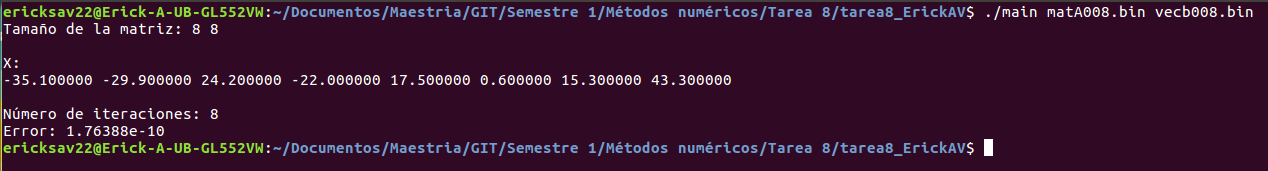
\includegraphics[scale=0.4]{E1.png}
	}\hfill
\end{figure}

\begin{figure}[H]
	\centering
	\subfloat[][Figura 2. Ejecución del algoritmo con un sistema de tamaño 100.]{
		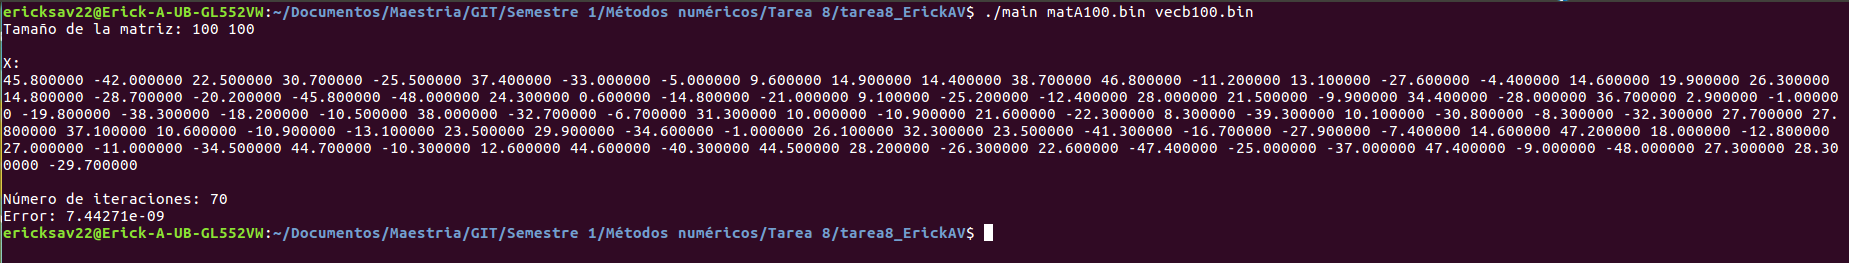
\includegraphics[scale=0.2]{E2.png}
	}\hfill
\end{figure}

En la Figura 1. podemos observar que el programa requiere hacer 8 iteraciones para encontrar el vector solución, mas aún en la Figura 2. observamos que para el sistema de tamaño 100 sólo se requieren 70 iteraciones, esto gracias a que se cumplió el criterio de convergencia.\\

\subsection{Compilación y ejecución}
\textbf{Para compilar:} En la carpeta encontraremos los archivos $.c$ y $.h$ con los que se podrá compilar el ejecutable. De la misma forma, en conjunto con los archivos anteriores, también podremos encontrar un Makefile para, en caso de encontrarse en linux, compilar de manera sencilla.

\begin{enumerate}
	\item \textbf{Compilar usando Makefile:} En la terminal, nos colocamos en el directorio donde se encuentre el programa, y ejecutamos el comando $make$, automáticamente se realizará la compilación y se generará el ejecutable. El Makefile también contiene el comando $make\ clean$ el cual limpiará los archivos generados por la compilación, incluyendo el ejecutable.
	\item \textbf{Compilar directamente:} De la misma forma, podemos compilar directamente usando los siguientes comandos (en terminal):
	\begin{itemize}
		\item gcc -c main.c
		\item gcc -c memo.c
		\item gcc -c reader.c
		\item gcc -c matriz\_vector.c
		\item gcc -c met\_num.c
		\item gcc -o main main.o memo.o reader.c matriz\_vector.o met\_num.o -lm
	\end{itemize}
\end{enumerate}

\textbf{Para ejecutar:} Únicamente debemos de usar el comando $./main$ para ejecutar el programa en consola, este recibe dos argumentos:
\begin{itemize}
	\item Un string: El nombre del archivo binario donde se encuentra la matriz.
	\item Un string: El nombre del archivo binario donde se encuentra el vector.
\end{itemize}

El programa ejecutará el método de gradiente conjugado en dicho sistema e imprimirá: el tamaño de la matriz, el vector solución $x^*$, el número de iteraciones realizadas y el valor del error.
\end{document}
